\newpage

\section{Skip Connection Neural Advection Model}
\label{sec:skipcon}

Our video prediction model, shown in ~\autoref{fig:prediction_model}, is inspired by the dynamic neural advection (DNA) model proposed by~\cite{finn_nips} and it is a variant of the SNA model proposed by~\cite{sna}. The model uses a convolutional LSTM~\cite{convlstm} to predict future frames. The prediction is initialized with an initial sequence of 2 ground truth frames, and predicts 13 futures frames. The model predicts these frames by iteratively making next-frame predictions and feeding those predictions back to itself. Each predicted frame, is given by a compositing layer, which composes intermediate frames with predicted compositing masks. The intermediate frames include the previous 2 frames and transformed versions them. To easily allow various transformations for different parts of the image, we predict 8 transformed frames, 4 of which are the transformed from the previous frame, and the other 4 from the frame of 2 steps in the past. These intermediate frames are then combined with compositing masks, which are also predicted by the convolutional LSTM. For simplicity, we collectively refer to these transformations as a single transformation $\hat{F}_{t+1 \leftarrow t}$ in~\autoref{simple_dna}. In addition, the first frame of the sequence is also given as one of the intermediate frames~\cite{sna}.

To enable action conditioning, the robot actions are also given to the generator. The action is passed to all the convolutional layers of the main network, by concatenating it along the channel dimension of the inputs of these layers. Since they are vectors with no spatial dimensions, they are replicated spatially to match the spatial dimensions of the inputs.

The SNA variant that we use incorporate the architectural improvements proposed by~\cite{savp}. Each convolutional layer is followed by instance normalization \cite{instancenorm} and ReLU activations. We also use instance normalization on the LSTM pre-activations (i.e., the input, forget, and output gates, as well as the transformed and next cell of the LSTM). In addition, we modify the spatial downsampling and upsampling mechanisms. Standard subsampling and upsampling between convolutions is known to produce artifacts for dense image generation tasks~\cite{odena2016deconvolution,Niklaus_ICCV_2017}. In the encoding layers, we reduce the spatial resolution of the feature maps by average pooling, and in the decoding layers, we increase the resolution by using bilinear interpolation. All convolutions in the generator use a stride of 1. The actions are concatenated to the inputs of all the convolutional layers of the main network, as opposed to only the bottleneck.

\begin{wrapfigure}{r}{.37\columnwidth}
	\centering
	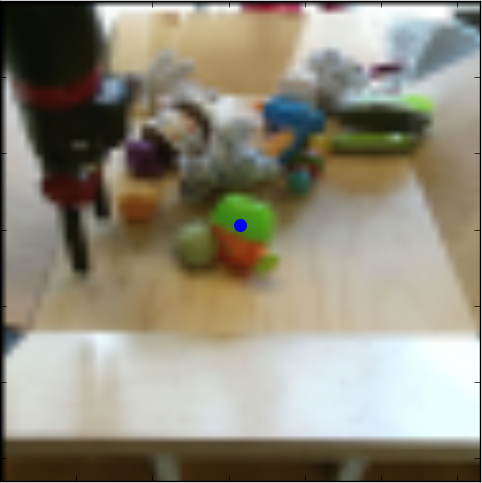
\includegraphics[width=0.37\columnwidth]{images_sna/occlusionaware/img_desigpixb0.png}
	\caption{The blue dot indicates the designated pixel}
	\label{fig:desig_pix_bluedot}
\end{wrapfigure}

We provide an example of the skip connection neural advection (SNA) model recovering from occlusion in \autoref{fig:pix_reappear}. In this figure, the arm is predicted to move in front of the designated pixel, marked in blue in \autoref{fig:desig_pix_bluedot}. The predictions of the DNA model, shown in figure \autoref{fig:pix_reappear}(b), contain incorrect motion of the marked object, as shown in the heatmaps visualizing $\hat{P}_t$, although the arm actually passes in front of it. This is because the DNA model cannot recover information about an object that it has `overwritten' during its predictions, causing the model to predict that the pixel \emph{moves with the arm}. We identified this as one of the major causes of planning failure using the DNA model. By contrast our SNA model predicts that the occluded object will not move, shown in figure  \autoref{fig:pix_reappear}(a).

\begin{figure}
	\centering
	\begin{subfigure}{0.9\columnwidth}
		\centering
		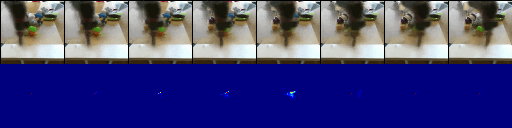
\includegraphics[width=1.\linewidth]{images_sna/occlusionaware/cdna_1ststep_bckgd_gen_pixb0_overtime.png}
		\caption{Skip connection neural advection (SNA) does not erase or move objects in the background}
		\label{fig:Ng1}
	\end{subfigure}
	\begin{subfigure}{0.9\columnwidth}
		\centering
		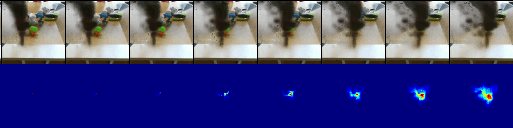
\includegraphics[width=1.0\linewidth]{images_sna/occlusionaware/orig_dna_gen_pixb0_overtime.png}
		\caption{Standard DNA \cite{foresight} exhibits undesirable movement of the distribution $P_{d}(t)$ and erases the background}
	\end{subfigure}
	\caption{
		%\protect\subref{fig:Ng1} 
		Top rows: Predicted images of arm moving \textit{in front of} green object with designated pixel (as indicated in \autoref{fig:desig_pix_bluedot}). 
		%(\protect\subref{fig:Ng2}) 
		Bottom rows: Predicted probability distributions $P_{d}(t)$ of designated pixel obtained by repeatedly applying transformations.}
	\label{fig:pix_reappear}
\end{figure}

\section{Improved Action Sampling Distributions for Data Collection}
\label{sec:folding_sampling}
In order to collect meaningful interaction data for learning folding of deformable objects such as towels and cloth, we found that the grasping primitive can be slightly adapted to increase the likelihood of encountering states where cloths are actually folded. When using actions sampled from a simple distribution or the previously-described distribution, clothing would become tangled up. To improve the efficiency of folding cloths we use an action primitive similar to the grasping primitive, but additionally we reduce lateral motion of the end-effector when the gripper is close to the table, thus reducing events where cloths become tangled up.

\section{Improvements of the CEM-Optimizer}
\label{sec:cem_improv}
In the model-predictive control setting, the action sequences found by the optimizer can be very different between execution real-world times steps. For example at one time step the optimizer might find a pushing action leading towards the goal and in the next time step it determines a grasping action to be optimal to reach the goal. Na\"{i}ve replanning at every time step can then result in alternating between a pushing and a grasping attempt indefinitely causing the agent to get stuck and not making any progress towards to goal. 

%%SL.10.15: It's not clear whether this is done in every experiment or just some experiments.
We can resolve this problem by modifying the sampling distribution of the first iteration of CEM so that the optimizer commits to the plan found in the previous time step. In the simplest version of CEM the sampling distribution at first iteration of CEM is chosen to be a Gaussian with diagonal covariance matrix and zero mean. We instead use the best action sequence found in the optimization of the \emph{previous} real-world time step as the mean for sampling new actions in the \emph{current} real-world time-step. Since this action sequence is optimized for the previous time step we only use the values $a_{2:T}$ and omit the first action. To sample actions close to the action sequence from the previous time step we reduce the entries of the diagonal covariance matrix for the first $T-1$ time steps. It is crucial that the last entry of the covariance matrix at the end of the horizon is not reduced otherwise no exploration could happen for the last time step causing poor performance at later time steps.

\section{Experimental Setup}
\label{sec:experiment_setup}
To train both our video-prediction and registration models, we collected 20,000 trajectories of pushing motions and 15,000 trajectories with gripper control, where the robot randomly picks and moves objects using the grasping reflex described in section \ref{sec:system}. The data collection process is fully autonomous, requiring human intervention only to change out the objects in front of the robot. The action space consisted of relative movements of the end-effector in cartesian space along the $x$, $y$, and $z$ axes, and for some parts of the dataset we also added azimuthal rotations of the gripper and a grasping action.

\section{Experimental Evaluation}

\begin{figure*}
    \centering    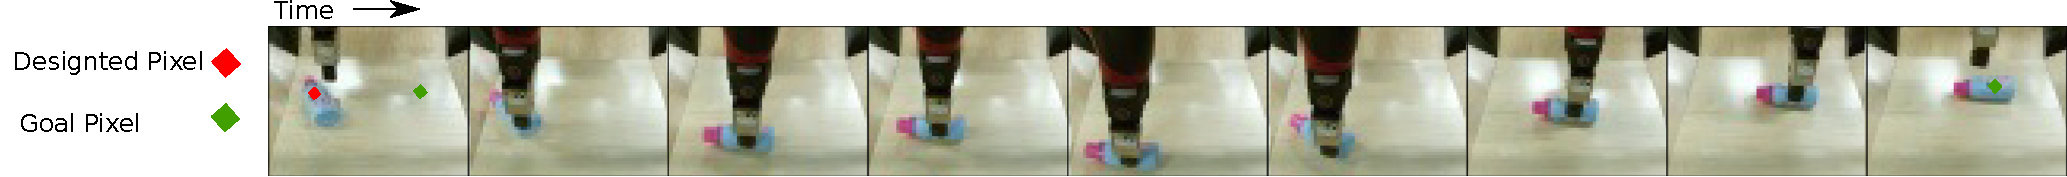
\includegraphics[width=1.0\textwidth]{images_rfr/push_correction.pdf}
    \caption{\small{Applying our method to a pushing task. In the first 3 time instants the object behaves unexpectedly, moving down. The tracking then allows the robot to retry, allowing it to eventually bring the object to the goal.}}
    \label{fig:push_retry}
\end{figure*}

\begin{figure*}
	\centering
	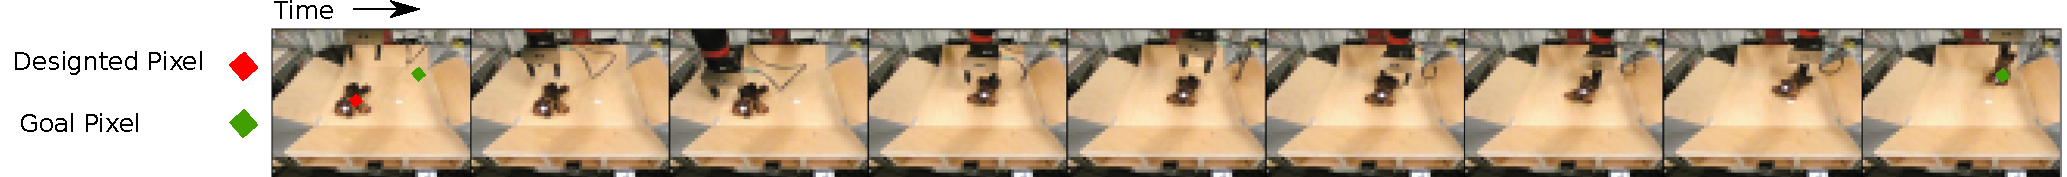
\includegraphics[width=1.0\textwidth]{images_rfr/pick_place_plush.pdf}
	\caption{\small{Retrying behavior of our method combining prehensile and non-prehensile manipulation. In the first 4 time instants shown the robot pushes the object. It then loses the object, and decides to grasp it pulling it all the way to the goal. Retrying is enabled by applying the learned registration to both camera views (here we only show the front view).}}
	\label{fig:push_grasp}
\end{figure*}

\subsection{Experiments with multiple-objects rearrangement with occlusion}

\autoref{fig:goingaroundocclusion} shows an example of the SNA model successfully predicting the position of the obstacle through an occlusion and finding a trajectory that avoids the obstacle. 

\begin{figure*}
	\centering
	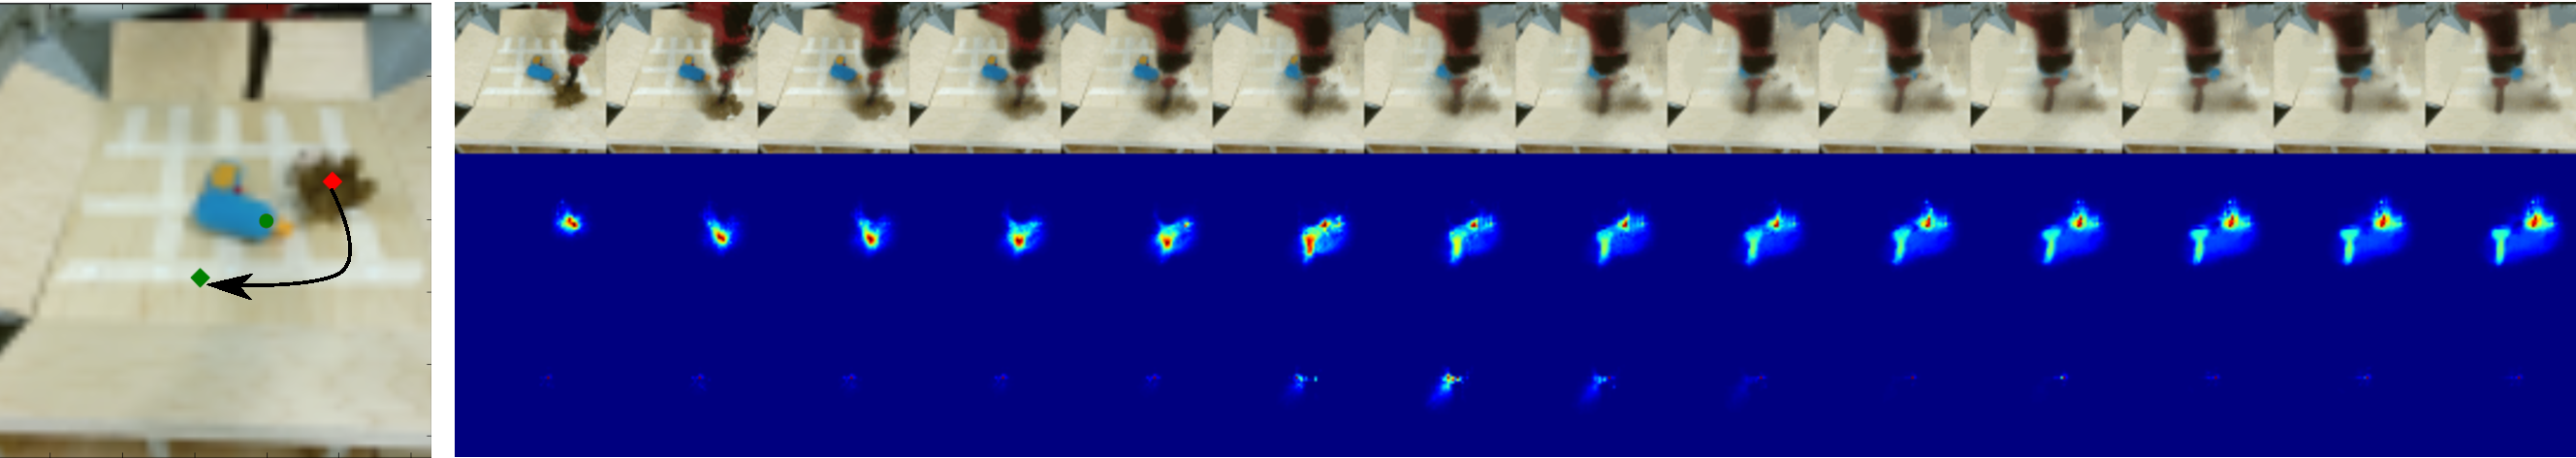
\includegraphics[width=1\linewidth]{images_sna/multiobject_qualitative/avoid_obstacle.pdf}
	\caption{Left: Task setup with green dot marking the obstacle. Right, first row: the predicted frames generated by SNA. Second row: the probability distribution of the designated pixel on the \textit{moving} object (brown stuffed animal). Note that part of the distribution shifts down and left, which is the indicated goal. Third row: the probability distribution of the designated pixel on the obstacle-object (blue power drill). Although the distribution increases in entropy during the occlusion (in the middle), it then recovers and remains on its original position.
		\label{fig:goingaroundocclusion}}
\end{figure*}


\section{Simulated Experiments}
%\todo{shorten if necessary}

In order to provide a more controlled comparison, we also set up a realistic simulation environment using MuJoCo \cite{todorov2012mujoco}, which includes a robotic manipulator controlled via Cartesian position control, similar to our real world setup, pushing randomly-generated L-shaped objects with random colors (see details in supplementary materials). 
We trained the same video prediction model in this environment, and set up 50 evaluation tasks where blocks must be pushed to target locations with maximum episode lengths of 120 steps. 
We  compare our proposed registration-based method, ``predictor propagation,'' and ground-truth registration obtained from the simulator, which provides an oracle upper bound on registration performance. 

%\autoref{fig:sim_bench} shows the results of this simulated evaluation, where the x-axis shows different distance thresholds, and the y-axis shows the fraction of evaluation scenarios where each method pushed the object within that threshold. We can see that, for thresholds around 0.1, our method drastically outperforms predictor propagation (i.e., prior work~\cite{sna}), and has a relatively modest gap in performance against ground-truth tracking. This indicates that our registration method is highly effective in guiding visual MPC, despite being entirely self-supervised.




